\section{Results}

For each episode, episode scores are calculated by summing up rewards of each time step. 
In \figref{fig:scatter_ep_rewards}, a scatter plot is visualized for each model's episode scores. 
In \figref{fig:std_ep_rewards}, moving average and standard deviation is visualized for each model's episode scores. 

\begin{figure}
	\centering
	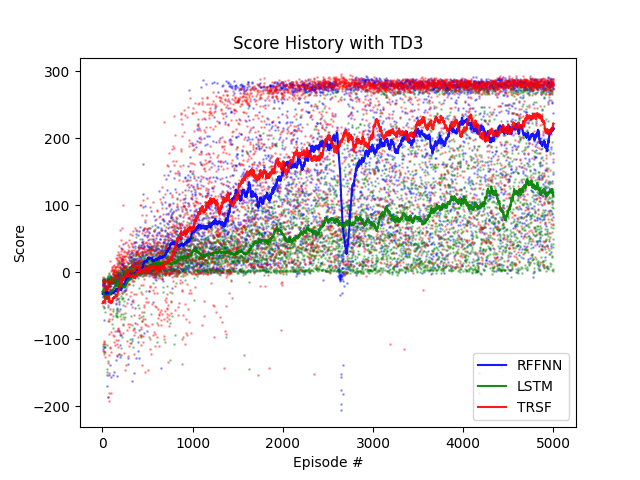
\includegraphics[width=0.95\textwidth]{figures/bipedal/SCATTER_TD3_RFFNN_LSTM_TRSF.png}
	\caption{Scatter Plot with Moving Average for Episode Scores}
	\label{fig:scatter_ep_rewards}
\end{figure}
\begin{figure}
	\centering
	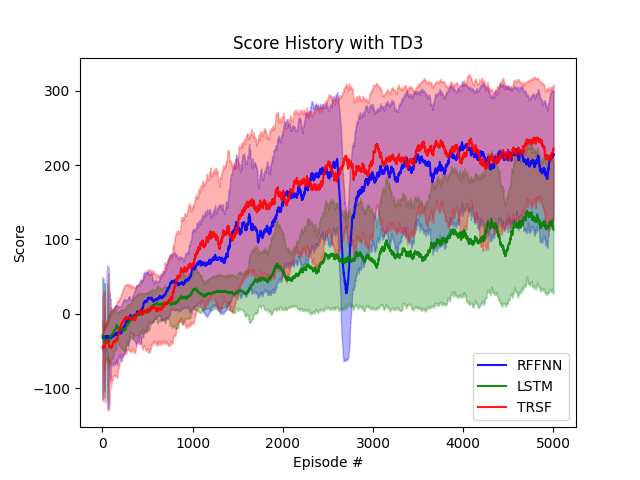
\includegraphics[width=0.95\textwidth]{figures/bipedal/STD_TD3_RFFNN_LSTM_TRSF.png}
	\caption{Moving Average and Standard Deviation for Episode Scores}
	\label{fig:std_ep_rewards}
\end{figure} 

First of all, none of our approaches solved the problem since 300 points required in 100 random simulations as solution. 
However, our methods partially solved problems by exceeding 200 point limit, while some simulations yield around 280 points in all models. 

RFFNN seems to be enough for solving the problem, although there exist partial observability in the environment. 
That model reaches around 220 points in average. 

The robot was able to walk by LSTM model but yield worse results and cannot exceed 120 points in average. 

Transformer model yield best results by reaching 230 points. 

As Transformer and RFFNN are relatively succesfull, their behavior is visualized in \figref{fig:rffnn_simulation} and \figref{fig:trsf_simulation}. 
The main behavior difference is when the agent faces with a big hurdle. 
First model passes it by jumping while other does by taking a very big step, shown in \figref{fig:anim_rffnn_hurdle} and \figref{fig:anim_trsf_hurdle}.

\begin{figure}
	\centering
	\begin{subfigure}{.9\textwidth}
		\centering
		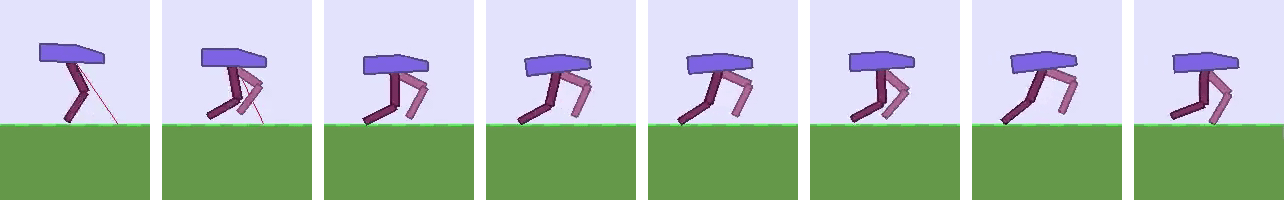
\includegraphics[width=0.99\textwidth]{figures/bipedal/anim/ff_flat.png}
		\caption{Flat Surface}
		\label{fig:anim_rffnn_flat}
	\end{subfigure}
	\begin{subfigure}{.9\textwidth}
		\centering
		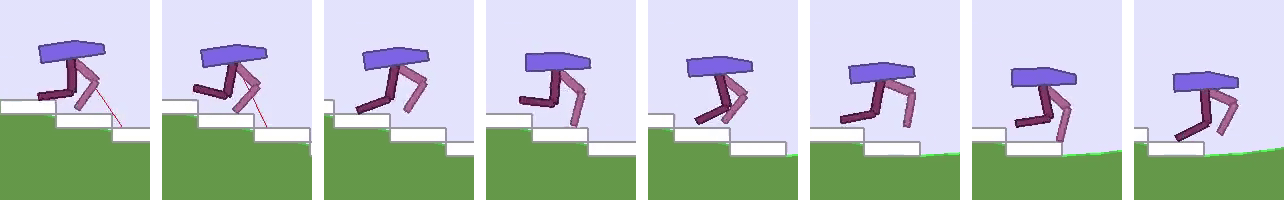
\includegraphics[width=0.99\textwidth]{figures/bipedal/anim/ff_stairs.png}
		\caption{Stairs}
		\label{fig:anim_rffnn_stairs}
	\end{subfigure}
	\begin{subfigure}{.9\textwidth}
		\centering
		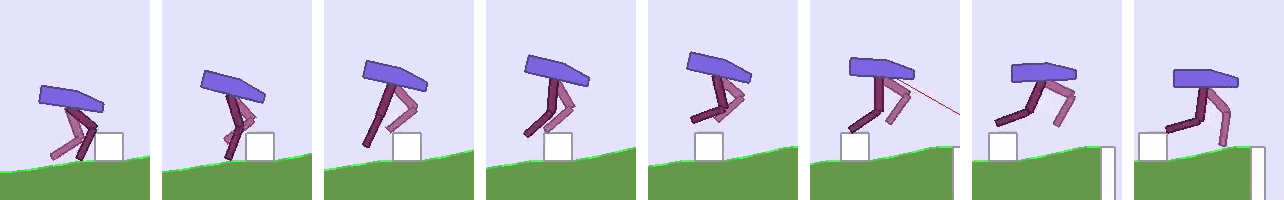
\includegraphics[width=0.99\textwidth]{figures/bipedal/anim/ff_hurdle.png}
		\caption{Hurdle}
		\label{fig:anim_rffnn_hurdle}
	\end{subfigure}
	\begin{subfigure}{.9\textwidth}
		\centering
		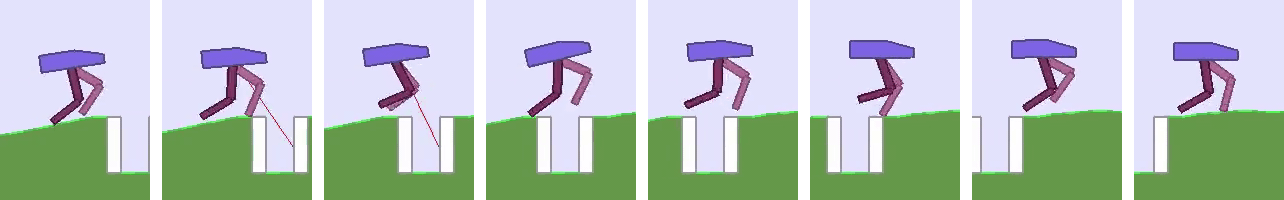
\includegraphics[width=0.99\textwidth]{figures/bipedal/anim/ff_pitfall.png}
		\caption{Pitfall}
		\label{fig:anim_rffnn_pitfall}
	\end{subfigure}
	\caption{Walking Simulation of RFFNN model at best version}
	\label{fig:rffnn_simulation}
\end{figure}

\begin{figure}
	\centering
	\begin{subfigure}{.9\textwidth}
		\centering
		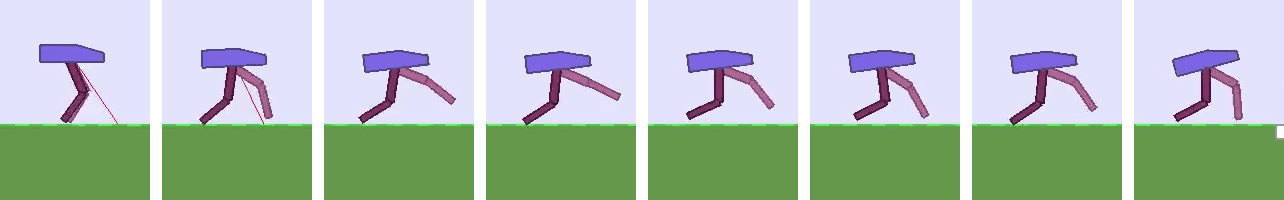
\includegraphics[width=0.99\textwidth]{figures/bipedal/anim/trsf_flat.png}
		\caption{Flat Surface}
		\label{fig:anim_trsf_flat}
	\end{subfigure}
	\begin{subfigure}{.9\textwidth}
		\centering
		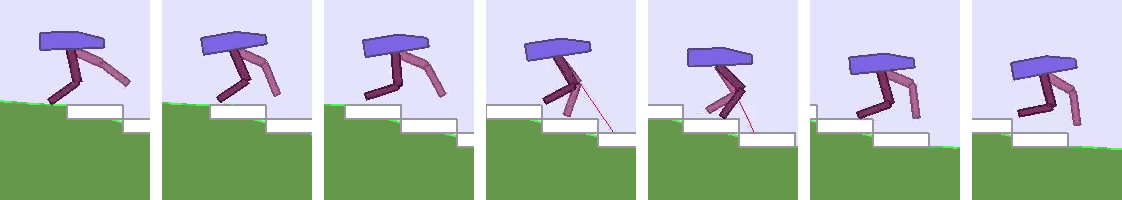
\includegraphics[width=0.99\textwidth]{figures/bipedal/anim/trsf_stairs.png}
		\caption{Stairs}
		\label{fig:anim_trsf_stairs}
	\end{subfigure}
	\begin{subfigure}{.9\textwidth}
		\centering
		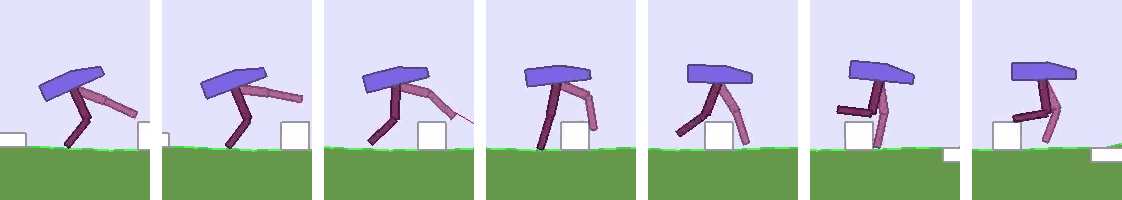
\includegraphics[width=0.99\textwidth]{figures/bipedal/anim/trsf_hurdle.png}
		\caption{Hurdle}
		\label{fig:anim_trsf_hurdle}
	\end{subfigure}
	\begin{subfigure}{.9\textwidth}
		\centering
		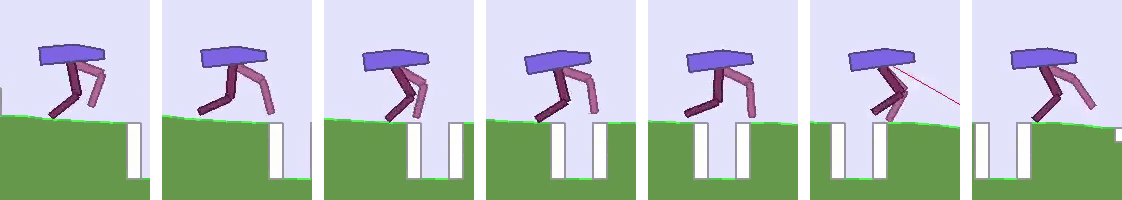
\includegraphics[width=0.99\textwidth]{figures/bipedal/anim/trsf_pitfall.png}
		\caption{Pitfall}
		\label{fig:anim_trsf_pitfall}
	\end{subfigure}
	\caption{Walking Simulation of Transformer model at best version}
	\label{fig:trsf_simulation}
\end{figure}
